%! Author = joels
%! Date = 27/01/2022

\section{Code Generierung}
\textbf{$\rightarrow$ Erzeugung von ausführbarem Maschinencode}\\
\textbf{Input:} Zwischendarstellung (Symboltabelle + AST)\\
\textbf{Output:} Maschinencode\\
\textbf{Mögliche Zielmaschinen:} Reale Maschine, (z.B. Intel 64, ARM Prozessor) oder virtuelle Maschine (z.B. Java VM, .NET CLI)\\
\textbf{Kernkonzepte:}
\begin{itemize}[topsep=0pt]
    \itemsep -0.2em
    \item Virtueller Stack-Prozessor (also keine Register)
    \item Branch Instructions (Goto) für Bedingungen wie if/while
    \item Metadaten wie z.B. Klassen, Methoden und Variablen die existieren
\end{itemize}
\subsection{Auswertungs-Stack}
\begin{itemize}[topsep=0pt]
    \itemsep -0.2em
    \item Instruktionen benutzen Auswertungs-Stack
    \item Jede Instruktion hat definierte Anzahl von Pop und Push Aufrufen
    \item Eigener Stack pro Methodenaufruf (Am Anfang und Ende leer)
    \item Stack hat unbeschränkte Kapazität
\end{itemize}

\begin{minipage}{0,5\linewidth}
    \subsubsection{Load/Store Numerierung}
    \begin{itemize}[topsep=0pt]
        \itemsep -0.2em
        \item this Referenz: Index 0 (virtuelle Methode)
        \item Danach n Parameters: 1..n
        \item Danach m lokale Variablen: Index n+1..n+m
    \end{itemize}
\end{minipage}
\begin{minipage}{0,5\linewidth}
    \begin{lstlisting}
  // Beispiel Instruktion imul:
  pop y
  pop x
  z = x * y
  push z
    \end{lstlisting}
\end{minipage}
\subsection{Metadaten}
Werden gebraucht für Fehlermeldungen, Allozieren von Speicher, Vererbung
\begin{itemize}[topsep=0pt]
    \itemsep -0.2em
    \item Zwischensprache kennt alle Informationen zu
    \SubItem{Klassen (Namen, Typen der Fields, Methoden)}
    \SubItem{Methoden (Namen, Parametertypen, Rückgabetyp)}
    \SubItem{Lokale Variablen (Typen)}
    \item Kein direktes Speicherlayout festgelegt
    \item Nicht enthalten:
    \SubItem{Namen von lokalen Variablen und Parameter $\rightarrow$ Sind nur nummeriert}
\end{itemize}

\subsubsection{Code-Generierung}
\begin{itemize}[topsep=0pt]
    \itemsep -0.2em
    \item Traversiere Symboltabelle
    \SubItem{Erzeuge Bytecode Metadaten}
    \item Traversiere AST pro Methode (Visitor)
    \SubItem{Erzeuge Instruktionen via Bytecode Assembler}
    \item Serialisiere in Output Format
\end{itemize}

\subsubsection{Traversierungsreihenfolge}
\begin{itemize}[topsep=0pt]
    \itemsep -0.2em
    \item Bei Expressions: Immer Post-Order
    \item Bei Statements: Je nach Code-Template
    \SubItem{Assignment: Rechts zuerst, dann Code Muster}
    \SubItem{If, If-Else, While etc. komplizierter}
\end{itemize}
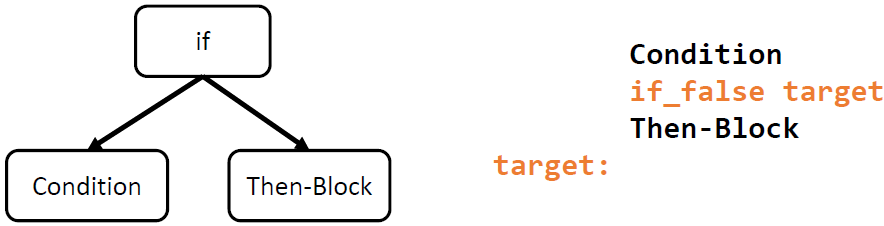
\includegraphics[width=0.7\linewidth]{if_statement}\\
\linebreak
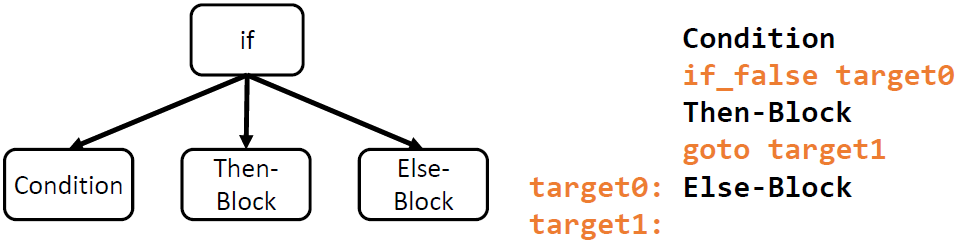
\includegraphics[width=0.7\linewidth]{if_else_statement}\\
\linebreak
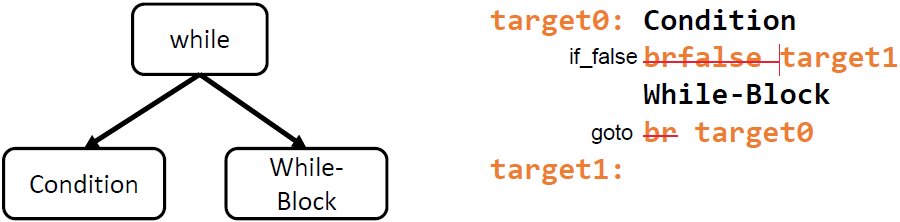
\includegraphics[width=0.7\linewidth]{while_statement}\\
\begin{lstlisting}
// While Statement
@Override
public void visit (WhileStatementNode node) {
    var beginLabel = assembler.createLabel();
    var endLabel = assembler.createLabel();
    assembler.setLabel(beginLabel);
    node.getCondition().accept(this);
    assembler.emit(IF_FALSE, endLabel);
    node.getBody().accept(this);
    assembler.emit(GOTO, beginLabel);
    assembler.setLabel(endLabel);
}
\end{lstlisting}

\subsubsection{Short Circuit}
\begin{lstlisting}
// a \&\& b
if a then b
else false

// a || b
if !a then b
else true
\end{lstlisting}

\subsection{Methodenaufrufe}
\begin{itemize}[topsep=0pt]
    \itemsep -0.2em
    \item Statisch
    \SubItem{Vordefinierte Methoden: readInt(), writeInt() etc.}
    \item Sonst immer virtuell (dynamisch)
    \SubItem{An Objekt gebunden z.B. x.run() oder this.run()}
\end{itemize}

\subsubsection{Virtueller Methodenaufruf}
\begin{enumerate}[topsep=0pt]
    \itemsep -0.2em
    \item Argumente von Methode sind auf dem Stack (letztes zuoberst), zuunterst ist Objektreferenz (this)
    \item Call-Instruktion
    \item Call entfernt Argumente \& Objektreferenz und legt Rückgabewert auf Stack (falls nicht void) $\rightarrow$ Assembler Code ret ist aber auch bei void-Methode nötig
\end{enumerate}